\section{Speicherklassen}
	\subsection{Adressraum eines Programms}
		\begin{minipage}[t]{10 cm}
			Der Adressraum eines ablauffähigen C-Programms - also einer Datei programm.exe - besteht aus den vier Segmenten: Code, Daten, Stack und Heap.\\\\
			\begin{minipage}[c]{4 cm}
				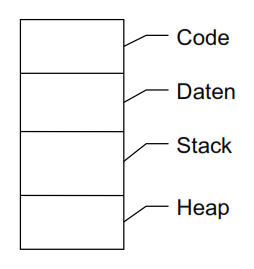
\includegraphics[width=1\textwidth]{pics/Adressraum.png}
			\end{minipage}
			\hspace*{0.5cm}
			\begin{minipage}[c]{5 cm}
				Codesegment:
				\begin{compactitem}
					\item Zugriff: lesen, ausführen
					\item im Flash EPROM oder im RAM (z.B. beim PC)
				\end{compactitem}
				\vspace*{0.5cm}
				Datensegment, Stack, Heap:
				\begin{compactitem}
					\item Zugriff: lesen und schreiben
					\item im RAM, evtl. in Registern
				\end{compactitem}				
			\end{minipage}
		\end{minipage}
		\hspace*{1cm}
		\begin{minipage}[t]{10 cm}
			\vspace*{-0.4cm} 
			\subsubsection{Code}
				\begin{compactitem}
					\item Programm in Maschinencode
				\end{compactitem}
			\subsubsection{Daten}
				\begin{compactitem}
					\item Globale Variablen, static Variablen
				\end{compactitem}		
			\subsubsection{Stack}
				\begin{compactitem}
					\item Lokale Variablen
					\item Parameter einer Funktion
					\item Rücksprungadressen
				\end{compactitem}		
			\subsubsection{Heap}
				\begin{compactitem}
					\item Dynamische Variablen\\
					(Speicherplatz wird erst zu\\ Laufzeit angefordert)
				\end{compactitem}		
		\end{minipage}
		\subsubsection{Anforderungen in grösseren Projekten}
			\begin{compactitem}
				\item Der gesamte Code soll in mehrere Dateien aufgeteilt werden können.
				\item Der Gültigkeitsbereich von Namen (Variablen, Typen, Funktionen) soll 
				möglichst klein sein, die Namen sollen nicht im ganzen Projekt abgestimmt
				werden müssen.
				\item Die Schnittstellen zwischen den einzelnen Teilen (Dateien) sollen möglichst
				klein sein $\rightarrow$ stark entkoppeln
			\end{compactitem}
			\subsubsection{Information Hiding}
				\begin{compactitem}
					\item Grundsatz: nur das gegen aussen preisgeben, das auch notwendig ist
					\item Interne Implementationsdetails nicht veröffentlichen $\rightarrow$ Funktionen, die in keiner weiteren Unit verwendet werden, sollen nur lokal bekannt sein
					\item Schnittstelle möglichst klein halten
				\end{compactitem}
\newpage
		\subsection{Programme aus mehreren Dateien}
			\subsubsection{Übersetzungsvorgang}	
				\begin{compactitem}
					\item Quelldateien werden getrennt übersetzt
					\item Der Compiler erzeugt aus jeder Quelldatei eine Objektdatei mit Maschinencode
					\item Eine Objektdatei ist nicht ausführbar, da die Adressen der Funktionen (und globalen Variablen), die in einer anderen Datei definiert sind, noch nicht bekannt sind
					\item Der Linker löst genau diese noch offenen Referenzen auf, indem er alle zum ausführbaren Programm gehörenden Objektdateien linked (deutsch: bindet)
					\item Der Linker meldet genau dann einen Fehler, wenn er eine noch offene Referenz nirgends gefunden hat, bzw. nicht auflösen konnte
				\end{compactitem}
			\begin{minipage}[t]{9 cm}
				\subsubsection{Sourcedatei (nur) compilieren}
					gcc -c foo.c\\
					\begin{compactitem}
						\item Dadurch entsteht noch kein ausführbares Programm, sondern nur die Dateifoo.o, der Objectcode
						\item Dies muss mit allen *.c - Dateien gemacht werden
					\end{compactitem}
			\end{minipage}
			\hspace*{0.5cm}
			\begin{minipage}[t]{9 cm}
				\subsubsection{Objectdateien linken}
					gcc  -o  prog.exe  foo.o  goo.o  main.o\\
					\begin{compactitem}
						\item Alle Objectdateien müssen gelinkt werden
					\end{compactitem}
			\end{minipage}\\\\
			\begin{minipage}[t]{9 cm}	
				\subsubsection{Buildprozess}
					Der Buildprozess beinhaltet alle Schritte, um ein ausführbares Programm zu erhalten.\\\\
					gcc -c foo.c\\
					gcc -c goo.c\\
					gcc -c main.c\\
					gcc -o prog.exe foo.o goo.o main.o\\\\
					Es wäre mühsam, wenn diese Befehle jedesmal neu eingetippt werden müssten. Deshalb wird in der Praxis oft ein Buildscript oder ein Buildtool eingesetzt, z.B. make oder ant.
			\end{minipage}
			\hspace*{0.5cm}	
			\begin{minipage}[t]{9 cm}
				\subsubsection{Abhängigkeiten zwischen Dateien}
					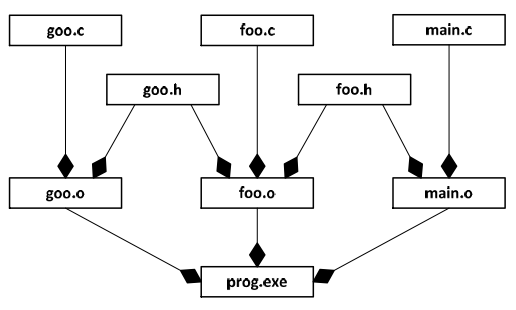
\includegraphics[width=0.9\textwidth]{pics/Abhaengigkeiten_Dateien.png}
			\end{minipage}\\\\
			\subsubsection{make-File}
				\begin{minipage}[c]{9 cm}
					\vspace*{-1.0cm}
					\begin{compactitem}
						\item In einem make-File können Abhängigkeiten definiert werden
						\item Wenn eine Datei geändert wurde, dann werden alle Operationen ausgeführt
						mit den Dateien, welche von dieser geänderten Datei abhängen 
						\item Der Befehl (gcc) wird z.B. nur dann ausgeführt, wenn sich an den Dateien, zu
						denen eine Abhängigkeit besteht, etwas geändert hat
					\end{compactitem}
				\end{minipage}
				\hspace*{0.5cm}
				\begin{minipage}[c]{9 cm}
					\vspace*{-0.6cm}
					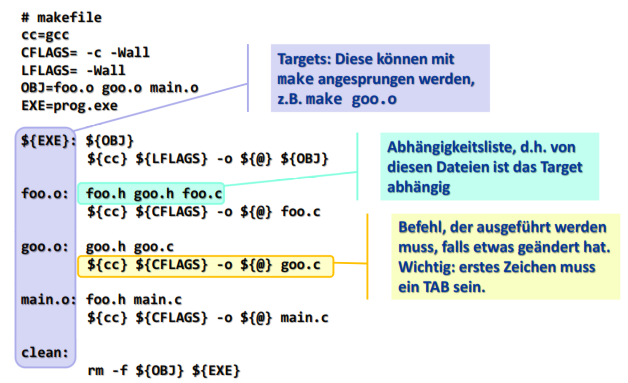
\includegraphics[width=0.9\textwidth]{pics/make_File.png}
				\end{minipage}
				\subsubsection{Feste vs. relokative Adressen}
					\begin{compactitem}
						\item Der Linker kann den Code auf feste physikalische (fixe) Adressen legen,\\
						oder
						\item auf virtuelle Adressen, welche erst beim Programmstart auf eine physikalische
						Adresse gelegt werden
					\end{compactitem}		
\newpage	
			\subsection{Speicherklassen extern}
				\begin{minipage}[c]{9 cm}
					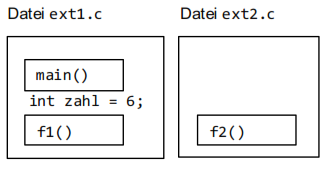
\includegraphics[width=0.7\textwidth]{pics/Speicherklasse_extern.png}\\
					// ext2.c\\
					extern int zahl; \ \ \ \ // zahl wird bekannt gemacht\\
					...
				\end{minipage}
				\hspace*{0.5cm}	
				\begin{minipage}[c]{9 cm}
					\vspace*{-0.4cm}
					\subsubsection{externe Variablen}
						\begin{compactitem}
							\item Eine externe Variable kann nur in einer einzigen Datei definiert werden (ohne
							extern)
							\item In den anderen Dateien wird sie mit extern deklariert (bekannt gemacht)
							\item Eine manuelle Initialisierung ist nur bei der Definition möglich
							\item Globale Variablen, welche nicht manuell initialisiert werden, werden
							automatisch mit 0 initialisiert
							\item extern-Deklarationen werden üblicherweise in einer Headerdatei deklariert. Am Beginn der .c - Datei wird die Headerdatei mit \#include eingefügt
						\end{compactitem}
				\end{minipage}	
			\subsection{Speicherklassen static}
				\begin{minipage}[t]{9 cm}
					\subsubsection{static Variablen}
					\begin{compactitem}
						\item static Variablen sind im Datenbereich, nicht auf dem Stack
						\item Gültigkeitsbereich ist der Block, in dem die Variable definiert ist
						\item static Variablen, welche ausserhalb einer Funktion definiert sind (globale Variablen), sind nur in der Datei gültig, in der sie definiert werden
						\item static Variablen sind nur einmal vorhanden (auch in Multithreading Umgebungen), d.h. ihr Wert wird erhalten, auch wenn die Funktion beendet ist. Beim nächsten Aufruf der Funktion geht es mit dem alten Wert weiter.
						\item Nur einsetzen, wenn man das will!\\
						$static$ $int$ $zahl$ $=$ $0$;
					\end{compactitem}
				\end{minipage}
				\hspace*{0.5cm}
				\begin{minipage}[t]{9 cm}
					\subsubsection{static Funktionen}
					\begin{compactitem}
						\item static Funktionen sind nur in der Datei, in welcher sie definiert sind,
						sichtbar
						\item Alle Funktionen, welche nicht aussen (für andere Units) sichtbar sein
						sollen, sollten deshalb als static definiert werden
						\item Mit anderen Worten: alle Funktionen static definieren, ausser jene, welche die Schnittstelle
						nach aussen bilden
					\end{compactitem}
				\end{minipage}
			\subsection{Speicherklassen bei lokalen Variablen}
				\subsubsection{Speicherklasse auto}
					\begin{compactitem}
						\item Variablen der Speicherklasse auto werden auf dem Stack angelegt
						\item Wenn bei einer Variablen keine Speicherklasse angegeben wird, so hat sie
						"automatisch" die Speicherklasse auto, d.h. auto ist der Default
						\item Die Speicherklasse auto wird praktisch nie explizit angegeben 
						\item Automatische Variablen werden beim Verlassen des Blocks, in dem sie
						definiert wurden, vom System automatisch aus dem Speicher entfernt
					\end{compactitem}
				\subsubsection{Speicherklasse register}
					\begin{compactitem}
						\item Bei Angabe der Speicherklasse register wird dem Compiler empfohlen, für
						diese Variable ein Register (schnellste Speicherzelle) zu verwenden
						\item Der Compiler wird dies versuchen, eine Garantie besteht aber nicht, da dem
						Compiler z.B. u.U. gar nicht genügend Register zur Verfügung stehen
						\item Bei formalen Parametern ist das die einzig mögliche explizite Speicherklasse
						\item Der Compiler optimiert meist gut, register soll deshalb üblicherweise nicht
						angegeben werden
					\end{compactitem}				
				\subsubsection{Speicherklasse static}
					\begin{compactitem}
						\item Wie bei allen Variablen der Speicherklasse static werden diese Variablen imglobalen Datenbereich (nicht auf dem Stack) angelegt
						\item Das einzige spezielle von lokalen static Variablen gegenüber globalen 
						static Variablen ist, dass die Sichtbarkeit auf den Block beschränkt ist, in
						welchem die Variable definiert ist
						\item Diese Einschränkung der Sichtbarkeit ist sehr zu begrüssen
					\end{compactitem}	
\newpage
				\subsubsection{Initialisierung}
					\begin{compactitem}	
						\item Automatische Variablen werden nicht durch das System initialisiert. Ihr Wert
						ist deshalb vor der manuellen Initialisierung undefiniert.
						\item Externe und statische lokale Variablen werden automatisch mit 0 initialisiert.
						Es ist guter Programmierstil, auch diese Variablen explizit zu initialisieren.
					\end{compactitem}		